\documentclass{article}
\usepackage{graphicx} % Required for inserting images
\usepackage{amsmath}        % Para símbolos matemáticos
\usepackage{algorithm}      % Entorno flotante para el algoritmo
\usepackage{algpseudocode}  % Comandos para escribir el pseudocódigo
\title{FANS}
\author{Samuel García}
\date{December 2025}

\begin{document}

\maketitle

\section{FANS}

Se trata de un método de búsqueda por entornos adaptativo y difuso, basado en cuatro componentes principales:
\begin{itemize}
    \item Operador: construye las soluciones.
    \item Valoración difusa: cualifica las soluciones.
    \item Administrador de operación: adapta el comportamiento o características del operador.
    \item Administrador de vecindario: 
\end{itemize}

De forma más matemática FANS queda definido por la septúpla $(NS,O,OS,\mu,Pars,(cond,accion))$, donde:
\begin{itemize}
    \item NS: administrador de vecindario.
    \item O: operador utilizado para construir soluciones.
    \item OS: administrador de operación.
    \item $\mu$: valoración difusa.
    \item Pars: conjunto de parámetros.
    \item (cond,accion): regla de tipo IF cond THEN accion que se utiliza para detectar y actuar en consecuencia cuando la búsqueda se ha estancado.
\end{itemize}

\subsection{Operador de Modificación}
El opeardor de modificación va a construir nuevas soluciones $s_i$ a partir de las soluciones anteriores $s$. Se define tal que $\mathcal{O}_i \in \mathcal{M}$, $\mathcal{O}_i : \mathcal{S} \times \mathcal{P} \rightarrow S$


\subsection{Valoración Difusa}

Las soluciones se evaluan mediante la función objetivo y una valoración difusa. Esta valoración difusa se define tal que:
$\mu \in \mathcal{F}$, con $\mu : \mathcal{R} \rightarrow [0,1]$. Esta valoración $\mu$ nos devuelve el grado de pertenencia de la solución al conjunto difuso.

\subsubsection{Utilidad}

La utilidad fundamental de la valoración difusa reside en su capacidad para modular el comportamiento global del algoritmo FANS. La definición de sus componentes y la interacción entre ellos permiten que el algoritmo emule diversas metaheurísticas clásicas simplemente ajustando la definición de \emph{aceptabilidad}.

Asumiendo un esquema de selección de tipo \emph{First} (donde se selecciona la primera solución vecina $\hat{s}$ tal que $\mu(s, \hat{s}) \ge \lambda$, siendo $\lambda$ un nivel mínimo de calidad), la valoración difusa permite adaptar la estrategia de búsqueda a los siguientes comportamientos clásicos en un problema de minimización:

\begin{itemize}
    \item \textbf{Caminos Aleatorios:}
    Si se considera cualquier solución del vecindario como aceptable, el algoritmo explora el espacio de búsqueda sin dirección preferente. Esto se logra definiendo una valoración constante máxima:
    \begin{equation}
        \mu(s, \hat{s}) = 1, \quad \forall \hat{s} \in N(s)
    \end{equation}
    De esta forma, cualquier solución generada es seleccionada, produciendo un comportamiento puramente estocástico.

    \item \textbf{Hill Climbing:}
    Para obtener un comportamiento de búsqueda local estricta, la valoración difusa debe restringir la aceptabilidad únicamente a aquellas soluciones que mejoran el costo actual. Fijando $\lambda = 1$, la función se define como:
    \begin{equation}
        \mu(s, \hat{s}) = 
        \begin{cases} 
            1 & \text{si } f(\hat{s}) < f(s) \\
            0 & \text{en otro caso}
        \end{cases}
    \end{equation}
    Bajo esta configuración, el algoritmo solo transita hacia soluciones mejores, terminando su ejecución al alcanzar un óptimo local.

    \item \textbf{Recocido Simulado:}
    Este método permite aceptar soluciones que empeoran la función objetivo con cierta probabilidad para escapar de óptimos locales. En FANS, esto se modela mediante una función de valoración que depende de un umbral de deterioro $\beta$:
    \begin{equation}
        \mu(s, \hat{s}) = 
        \begin{cases} 
            0 & \text{si } f(\hat{s}) > \beta \\
            \frac{\beta - f(\hat{s})}{\beta - f(s)} & \text{si } f(s) \le f(\hat{s}) \le \beta \\
            1 & \text{si } f(\hat{s}) < f(s)
        \end{cases}
    \end{equation}
    Aquí, $\beta$ actúa como un límite de aceptabilidad. Si $\beta$ se define como una función dinámica $h(s, \hat{s}, t)$ que depende del tiempo o del número de iteraciones $t$, es posible reducir el deterioro aceptable a medida que la búsqueda progresa (enfriamiento), convergiendo finalmente hacia un comportamiento donde solo se aceptan mejoras.
\end{itemize}

En conclusión, mediante la variación de $\mu$ y los parámetros asociados, la valoración difusa transforma a FANS en un algoritmo de umbral adaptable capaz de replicar la dinámica cualitativa de métodos de búsqueda local consolidados.

\subsection{Administrador de Operación}

El administrador de Operación $\mathcal{OS}$ es el responsable de definir el orden de aplicación de los diferentes operadores utilizados.
$\mathcal{OS}(\mathcal{O}^{ti}) \Rightarrow \mathcal{O}^{tj}$. Otra opción es disponer de un conjunto de operadores de modificación $\{\mathcal{O}_1, \mathcal{O}_2,\ldots,\mathcal{O}_k\}$ donde el Administrador puede escoer el orden de operación de los mismos.

\subsection{Administrador de Vecindario}
El Administrador del vecindario $\mathcal{N}$ es el responsable de generar nuevas soluciones. Su definición matemática es 
$\mathcal{NS}:\mathcal{S}\times\mathcal{F}\times\mathcal{M}\times\mathcal{P}\rightarrow\mathcal{S}$. Este vecindario puede ser:
\begin{itemize}
    \item Operativo: $\mathcal{N}(s) = \{ \hat{s}_i \mid \hat{s}_i = \mathcal{O}_i(s) \}$
    \item Semántico: $\hat{\mathcal{N}}(s) = \{ \hat{s}_i \in \mathcal{N}(s) \mid \mu(\hat{s}_i) \geq \lambda \}$. Las soluciones adecuadas son las que superen un cierto $\lambda$
\end{itemize}

\subsection{Parámetros globales}

El algoritmo mantiene un conjunto $Pars \in \mathcal{P}$ para llevar un registro de los estados de la búsqueda. Este conjunto es utilizado

\section{Algoritmo}

En cada iteración se comienza con una llamada al administrador de vecindario $\mathcal{NS}$ con los parámetros $\mathcal{S}_{cur}$, que representa la solución actual, $\mu$, valoración difusa, y $\mathcal{O}$, operador de modificación.

El resultado de la ejecución del administrador da lugar a dos posibles situaciones: se ha encontrado la solución óptima, en términos de $\mu$ o no.
En el primer caso esa solución obtenida pasa a ser la nueva solución actual y los parámetros de $\mu$ son adaptados.
En caso contrario, se aplica un mecanismo de escape, donde se ejecuta el administrador de operación $\mathcal{OS}$, con el objetivo de devolver una versión modificada del operador $\mathcal{O}$, lo que influirá en la búsqueda de soluciones.

Por último, existe una condición para evitar el estancamiento. Si se han utilizado varios operadores distintos y no se ha obtenido ninguna mejora, se evaluará el costo de la nueva solución y se adaptará la valoración difusa, reiniciando posteriormente la búsqueda.

El algoritmo finaliza cuando el número de
evaluaciones de la función de costo alcanza
cierto límite o cuando se realizó un número
predeterminado de evaluaciones.

El pseudocódigo es el siguiente:

\begin{algorithm}
\caption{Procedimiento FANS}
\begin{algorithmic}[0] % El [0] quita la numeración de líneas. Pon [1] si quieres numerarlas.

\State \textbf{Begin}
    \State \quad /* $\mathcal{O}$ : el operador de modificacion */
    \State \quad /* $\mu()$ : la valoracion difusa */
    \State \quad /* $S_{cur}, S_{new}$ : soluciones */
    \State \quad /* NS: el administrador de vecindario */
    \State \quad /* OS: el administrador de operacion */
    
    \State Inicializar Variables();
    
    \While{ ( \text{not-fin} ) }
        \State /* Ejecutar Admin. de Vecindario NS */
        \State $S_{new} = \text{NS}(S_{cur}, \mu(), \mathcal{O})$;
        
        \If{ ($S_{new}$ es ``buena'' en base a $\mu()$) }
            \State $S_{cur} := S_{new}$;
            \State adaptar-Valoracion-Difusa($\mu(), S_{cur}$);
        \Else
            \State /* Fue imposible hallar una $S_{new}$ ``buena'' 
            \State \quad con el operador $\mathcal{O}$ : Sera modificado */
            \State $\mathcal{O} := \text{OS-ModificarOperador}(\mathcal{O})$;
        \EndIf
        
        \If{ (HayEstancamiento?()) }
            \State Escape();
        \EndIf
    \EndWhile
\State \textbf{End.}

\end{algorithmic}
\end{algorithm}


\section{FANS como Heurística de Propósito General}

Más allá de su capacidad para mimetizar métodos clásicos, FANS se constituye como un \emph{framework} de optimización en sí mismo. Su mayor fortaleza radica en que la valoración difusa ($\mu$) no es simplemente una función matemática, sino que modela el \textbf{criterio de un decisor} ante el problema.

Esta flexibilidad permite definir curvas de aceptabilidad personalizadas que reflejan estrategias de búsqueda complejas, imposibles de configurar en algoritmos rígidos. A continuación se describen tres perfiles de decisión que ilustran esta capacidad:

\begin{center}[h]
    \begin{figure}
        \centering
        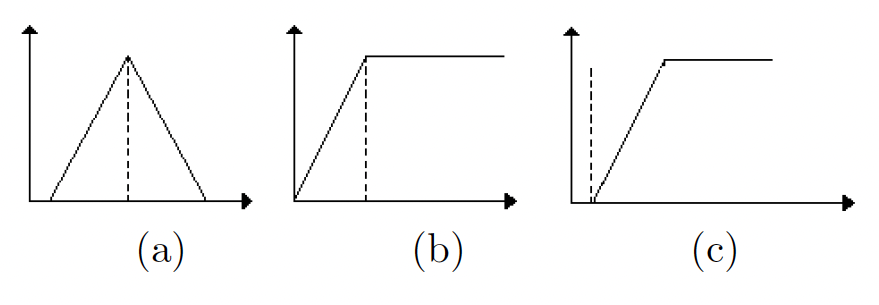
\includegraphics[width=0.8\linewidth]{img/formas.png}
        \caption{Ejemplo de variaciones difusas.} 
        \label{fig:placeholder}
    \end{figure}
\end{center}

\begin{itemize}
    \item \textbf{Criterio de Diversificación:} 
    Representa a un decisor que busca soluciones de costo similar a la actual ($f(\hat{s}) \approx f(s)$) pero diferentes en estructura. Es ideal cuando existen criterios cualitativos difíciles de cuantificar (como aspectos estéticos), permitiendo generar un abanico de alternativas equivalentes en costo antes de tomar una decisión final.
    
    \item \textbf{Criterio de Insatisfacción:} 
    Refleja la postura de un decisor que no tolera la solución actual. La valoración difusa asigna el máximo grado de aceptabilidad a cualquier opción que ofrezca una mejora, incentivando cambios rápidos en la trayectoria de búsqueda.
    
    \item \textbf{Criterio Conservador:} 
    Corresponde a un decisor reacio al cambio. Para que una nueva solución desplace a la actual, no basta con una mejora marginal; se exige que la mejora sea considerable y sustancial.
\end{itemize}

Adicionalmente, la potencia de FANS se ve amplificada por la posibilidad de aplicar \textbf{modificadores lingüísticos} (como \emph{muy} o \emph{algo}) sobre las definiciones de valoración, permitiendo un ajuste fino del comportamiento del algoritmo. 

En síntesis, FANS permite variar la estrategia de exploración de forma intuitiva y comprensible. Dado que diferentes topologías de problemas requieren diferentes estrategias de búsqueda para obtener resultados óptimos, esta capacidad de adaptación convierte a FANS en una herramienta genérica de optimización sumamente robusta.


\end{document}
